\renewcommand\chaptername{}
\chapter{BACKGROUND LITERATURE}

Forest inventory-related research papers have increased significantly in the last decade because of the rapid development of computational capacity and availability of high-resolution remote sensing imagery. The detection and delineation of \gls{ITC}s from remote sensing imagery is one of the initial steps needed to perform forest inventory on a bigger scale. For instance, delineated tree crowns can be used in object-based image analysis and classification, giving necessary information about the number of trees, size of the crowns, geolocation, forest type and tree species. Accurate tree delineation increases the classification rates for specie recognition, since it improves spectral signature characterization of individual trees by reducing the number of pixels, representing the tree crown \cite{Wagner2018}. Moreover, additional features, such as textural information and reflectance distributions, could be obtained from the data.

\begin{figure}[ht]
\centering
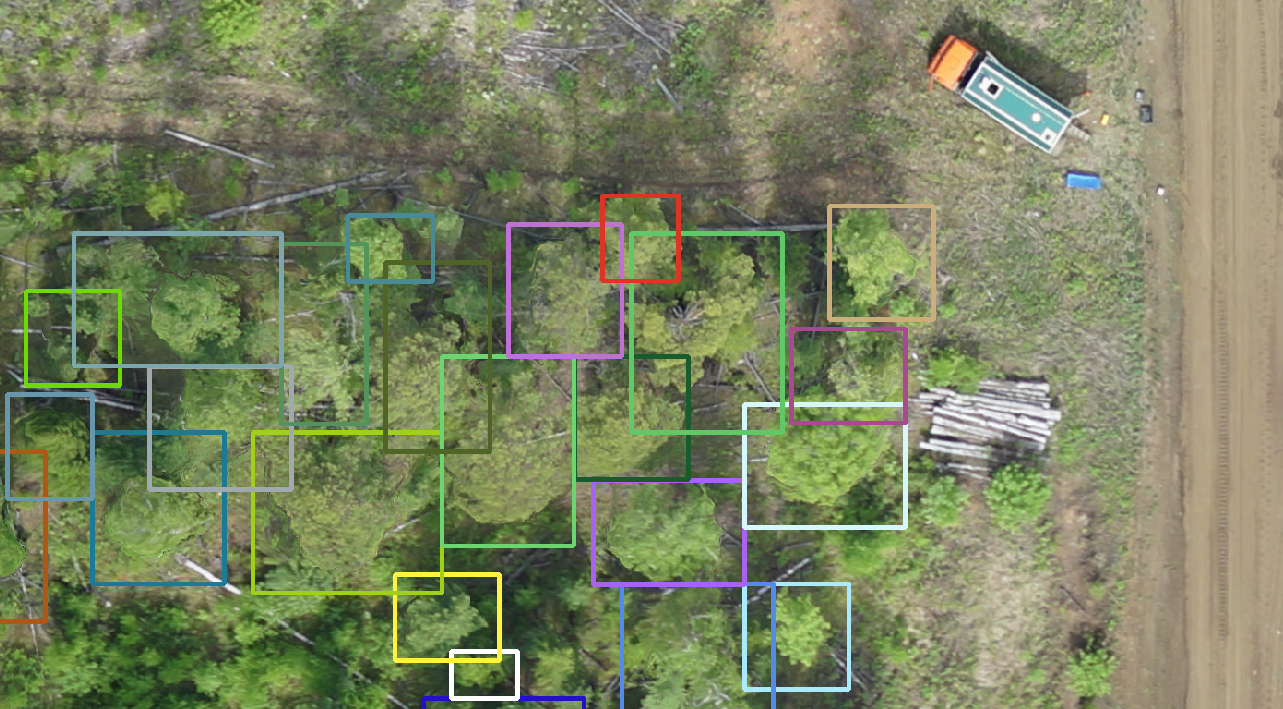
\includegraphics[scale=0.3]{images/ObjDet.png}
\caption{Example of ITC detection}
\label{ObjDet}
\end{figure}

\section{UAV-carried systems}

Currently, it is possible to obtain and analyze the data on a sub-stand level from Unmanned aerial vehicles (\gls{UAV}s) with multispectral and Light detection and ranging sensors (\gls{LIDAR}). There has been a decent amount of research related to forest inventory tasks with the mentioned devices, since UAVs with multispectral and LIDAR cameras become a better alternative to Airborne laser scanning (\gls{ALS}) in terms of density of point clouds, cost, and flexibility \cite{Hamraz2019}. Characteristics of individual tree structures, such as crown size, height, can be obtained from the segmented trees.

\section{\gls{ITC} delineation methods}

Several approaches of \gls{ITC} delineation were proposed in the articles. The first type of data used for tree segmentation is 2D raster images, which is called Digital elevation model (\gls{DEM}). \gls{DEM} data can be either Digital surface model (\gls{DSM}) or Canopy height model (\gls{CHM}). \gls{CHM} represents the distance between the top surfaces of trees and the terrain for every pixel in the raster image, so basically it shows the real height of the trees, while \gls{DSM} represents only top part of the surface (Fig. \ref{DEM}). The second data type uses 3D \gls{LIDAR} point clouds to extract the tree crown information. Regardless of the data type, tree delineation approaches can be classified as parametric and non-parametric \cite{Hamraz2016}.

\begin{figure}[ht]
\centering
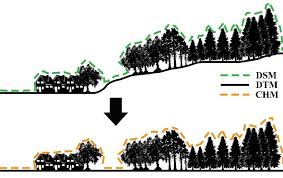
\includegraphics[scale=1.2]{images/DEM.png}
\caption{Representation of DEM}
\label{DEM}
\end{figure}

Parametric methods perform multi-stage filtering from the 3D points, where the filtering is based on our prior assumptions about the tree crown geometry. These methods include rule-based distance and height thresholding, voxel-, graph-, or kernel-based approaches \cite{Xiao2019}. The parameters of these methods are selected manually based on the field assessment of the forest structure and tree crown shapes. For instance, the Mean shift method, which was originally used for clustering the raster data, was adapted for direct 3D point cloud data segmentation by seeking the mode in feature space \cite{Michel2015}. The mode represents the maxima density function, it can be found by shifting the weighted mean determined by predefined kernel. Since the kernel can be extended into 3D space, the mean also can be calculated from the 3D point clouds. Due to this particular ability to go through the 3D space, the above-mentioned methods demonstrated good results for various forest types, such as boreal coniferous, mixed-species, or multi-layered forests \cite{Xiao2019}. Hamraz et al. suggest that these methods give better results in comparison to the 2D Digital elevation model \cite{Hamraz2016}. However, there are limitations due to the fact that these methods need predefined parameters (kernel shape and size, weighting parameters).

Non-parametric methods find the tree apexes, which are the Local maxima (\gls{LMX}) in the raster image, or Local minima (\gls{LM}), which correspond to boundaries between trees. By applying \gls{LMX} methods top of tree crown can be found within neighborhood area, followed by region-growing or clustering methods. The drawback is that it might be challenging to identify proper kernel size, due to varying tree crown sizes, or spatial resolutions \cite{Jing}, thus it can easily lead to loss of some tree crowns in image. Regression models based on tree heights of the region can be used to adaptively change the kernel size \cite{Hamraz2016}, but good results are obtained mostly from the coniferous forest, where tree crowns are homogeneous. The newer approaches use the non-parametric segmentations with a variety of kernel sizes, which creates a number of segmentation maps at different scales. After that, the results are interpreted based on the proposed scoring system \cite{Hamraz2016}.

Local minima (\gls{LM}) based approaches usually use watershed, region growing, hill climbing, and valley following algorithms \cite{Mosin2019, Gomes2018}. 

The template-matching algorithm compares the spectral characteristics of sample tree with the pixels by sliding through the image, which is not applicable to deciduous forest due to the variability of tree crown size and shape. 

Watershed segmentation is the most widely used algorithm, which has problems with under- or over- segmentation mainly due to the changing vegetation indices inside the tree crown area. This can be tackled by marker-controlled watershed algorithm, where the tree apexes are marked in advance prior to the actual delineation procedure. Since manual annotation of tree apexes is inefficient and time-consuming, the problem is solved by applying different mathematical morphological operations \cite{Hamraz2016}. Combination of Local maxima (\gls{LMX}) and watershed algorithm (LM) performed well, and gave better results in this particular research.

Non-parametric methods described above are mostly applied to coniferous or sparse forests, where certain assumptions can be made about tree and forest type \cite{Zaforemska2019}. These factors impose limitations to the variability of trees, and shall be carefully applied to deciduous forest. Increasing number of species, dense forest structure, changing tree sizes and shape, and overall complex vegetation conditions of deciduous forests challenge the application of \gls{ITC} delineation algorithm. The literature suggests that the aforementioned methods' performance radically varies (tree detection rate from 50\% to 90\%) depending on forest conditions \cite{Hamraz2016}. In addition, these methods are weakly generalizable on larger scales, since the parameters are tuned for distinct forest type, which confirms the need for a superior approach, which can be applied to different forest types while ensuring solid \gls{ITC} delineation results.

\section{Deep Learning in Forest Inventory}

Deep learning is state-of-the-art method for object detection and segmentation in RGB images, however it has only recently been applied to remote sensing data \cite{Weinstein2019}. The main benefit of this approach is in Convolutional neural network's \gls{CNN} ability to automatically calculate and obtain the needed features and parameters, with nominal prior information about the task.

In the case of image segmentation task, initial data is only provided as original images and ground truth masks of the objects for training. This approach is commonly used for land cover, scene classification and object extraction \cite{Wagner2018, Wagner2019}. In the field of remote sensing, deep learning-based applications are at the beginning, there are few, but perspective applications, such as tree delineation, as well as tree type classification \cite{Li2017}, however the spatial resolutions of the training data in the most of the papers was considerably higher than the satellite imagery resolution. 

The authors in this article \cite{Weinstein2019} used the \gls{LIDAR}-based methods to obtain the training set for \gls{ITC} delineation neural network model. Despite drawbacks of \gls{LIDAR}-based unsupervised delineation method, described in the previous section, the deep neural network was successfully trained on the noisy dataset. Using Intersection Over Union (\gls{IoU}) threshold set to 0.5, results obtained from the trained model were: 0.69 recall, 0.61 precision, and 0.82 tree detection rate for manually annotated test data. Tree detection is considered to be correct if manually labeled tree apex point lies inside the predicted bounding box. This is logically more suitable approach in comparison to other researches, where, for example, tree detection is considered to be correct if an edge of the bounding box lies within search radius. Because of these differences in measurement approaches, it was hard to locate the best performance, but overall 60\%-80\% tree detection rate between the ground truth and predicted trees is typical \cite{Xiao2018, Xiao2019, Narasipura2017, Wagner2019, Khan2018, DosSantos2019, Hamraz2019, Li2017, Weinstein2019, Guirado2017}.

However, in spite of all of the advantages of DL methods, the need for large and diverse training dataset is still the biggest problem. One approach to tackle this problem proposed by Weinstein et al. was to use “semi-supervised learning” approach, where firstly unsupervised methods are applied to gather initial training dataset \cite{Weinstein2019}. It was recently applied to remote sensing for hyperspectral image classification. Combination of unlabeled and labeled data represents semi-supervised approach, which can leverage the results of deep neural networks trained on a limited amount of data. The model obtains the initial generalized features on a wide range of training samples, and then can be retrained on a smaller, but high quality dataset. In detail, the semi-supervised pipeline for \gls{ITC} detection developed by Weinstein et al. proposes the following steps: first, \gls{LIDAR} unsupervised algorithm produces low quality tree crowns segmentation maps, which was used for initial training. Following this, the model is then retrained on smaller manually annotated data to improve the model parameters. As a result, the combination of differently obtained data: by unsupervised methods and manual delineation, allows the model to obtain good quality segmentation maps from new unseen RGB imagery \cite{Weinstein2019}. The problem arising from the lack of datasets is that the performance of the model will severely depend on the region, and results will change among different environments \cite{Weinstein2019}. However, the availability of UAV-carried multispectral or \gls{LIDAR} sensors will lead to cost-efficient acquisition of datasets from different regions. Overall, it can be concluded that growing use of \gls{UAV}s in remote sensing grants promising opportunities for combining very high resolution local data with large scale imagery obtained from satellites.

\section{\gls{ITC} Classification}

The results of individual tree crown detection and delineation (\gls{ITC}d) can be applied in forest classification, a particular case of land cover classification \cite{Mosin2019}. In general, any land cover classification task can be categorized either as pixel-based or as object-based, but the latter usually shows better results \cite{Pouliot2002}. Moreover, in forestry applications object-based tree species classification is preferable, since it gives more detailed information about a forest structure. There are two approaches for object-based forest classification: classification at the individual tree level, classifying every tree separately, or area-based classification, when dominant tree species are predicted for different areas of a forest. Forestry legislation seeks to obtain information for each tree rather than general statistics for whole parcels of a forest, thus the case of individual tree level forest species classification is more valuable. 